\documentclass{article}
\usepackage{amsmath, sfmath, pgfplots, multicol}
\pgfplotsset{compat = newest}
\usepgfplotslibrary{statistics}
\usepackage[margin = 0.5in]{geometry}
\renewcommand{\familydefault}{\sfdefault}
\setlength\parindent{0cm}
\pagestyle{empty}

\newcounter{pset}
\newcounter{key}


\begin{document}

\subsection*{Qualitative Graphs P-Set}

The frequency chart below describes the highest level of education for a group of surveyed randomly selected adults in the United States.

\begin{center}
\begin{tabular}{c|c}
    \textbf{Educational Attainment} & \textbf{Frequency} \\ \hline 
    No high school diploma & 12 \\
    High school graduate & 32 \\
    Some college & 39 \\
    Associate's degree & 43 \\
    Bachelor's degree & 36 \\
    Advanced degree & 25
\end{tabular}
\end{center}

\begin{enumerate}
    \item How many total adults were surveyed?
    \item Create a column for the relative frequencies as percents. Round to 2 decimal places for your percents.
    \item What percent of adults surveyed have a bachelor's degree?
    \item What percent of adults surveyed have only a high school diploma?
\end{enumerate} \setcounter{pset}{\value{enumi}}

\vfill

The graph below displays the frequencies of rehabilitation for a physical therapist's office.

\begin{center}
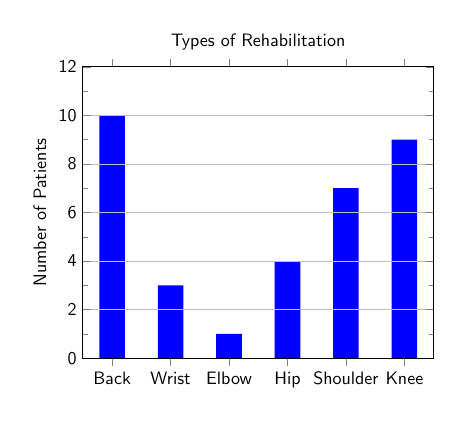
\begin{tikzpicture}[scale=0.65]
\begin{axis}[
ybar, axis on top, title={Types of Rehabilitation}, bar width = 0.5cm, ymajorgrids,
ymin = 0, ymax = 12, ylabel = {Number of Patients},
symbolic x coords = {Back, Wrist, Elbow, Hip, Shoulder, Knee}, xtick=data, minor y tick num = 1
]
\addplot [draw=none, fill=blue] coordinates{
(Back, 10) (Wrist, 3) (Elbow, 1) (Hip, 4) (Shoulder, 7) (Knee, 9)
};
\end{axis}
\end{tikzpicture}
\end{center}

\begin{enumerate}   \setcounter{enumi}{\value{pset}}
    \item If each patient is only seen for one type of injury, how many total patients are involved?
    \item What percent of total injuries involve the back?
    \item How many more injuries involve the knee than the hip?
    \item Create a relative frequency bar plot of the graph above.
\end{enumerate}     \setcounter{pset}{\value{enumi}}

\vfill 

The colors of twenty randomly selected luxury cars and twenty randomly selected sports cars are displayed below.

\begin{center}
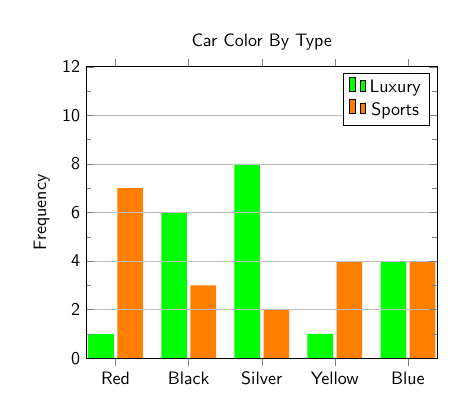
\begin{tikzpicture}[scale=0.65]
\begin{axis}[
ybar, axis on top, title={Car Color By Type}, bar width = 0.5cm, ymajorgrids,
ymin = 0, ymax = 12, ylabel = {Frequency}, legend entries = {Luxury, Sports},
symbolic x coords = {Red, Black, Silver, Yellow, Blue}, xtick=data, minor y tick num = 1
]
\addplot [draw=none, fill=green] coordinates{
(Red, 1)
(Black, 6)
(Silver, 8)
(Yellow, 1)
(Blue, 4)
};
\addplot [draw=none, fill=orange] coordinates{
(Red, 7)
(Black, 3)
(Silver, 2)
(Yellow, 4)
(Blue, 4)
};
\end{axis}
\end{tikzpicture}
\end{center}

\begin{enumerate}   \setcounter{enumi}{\value{pset}}
    \item How many more red sports cars are in the sample than silver sports cars?
    \item How many total yellow and blue luxury cars are in the sample?
    \item What percent of the luxury cars are black?
    \item Create a stacked bar graph for the clustered bar graph shown.
\end{enumerate}     \setcounter{pset}{\value{enumi}}

\newpage 

\texttt{Key}

\begin{enumerate}
    \item 187
    \item \mbox{} \newline\\
    \begin{tabular}{c|c|c}
    \textbf{Educational Attainment} & \textbf{Frequency} & \textbf{Relative Frequency} \\ \hline 
    No high school diploma & 12 & 6.42\% \\
    High school graduate & 32 & 17.11\% \\
    Some college & 39 & 20.86\% \\
    Associate's degree & 43 & 22.99\% \\
    Bachelor's degree & 36 & 19.25\% \\
    Advanced degree & 25 & 13.37\%
    \end{tabular}
    \item 19.25\%
    \item 17.11\%
    \item 34
    \item about 29.41\%
    \item 5
    \item \mbox{} \newline\\
    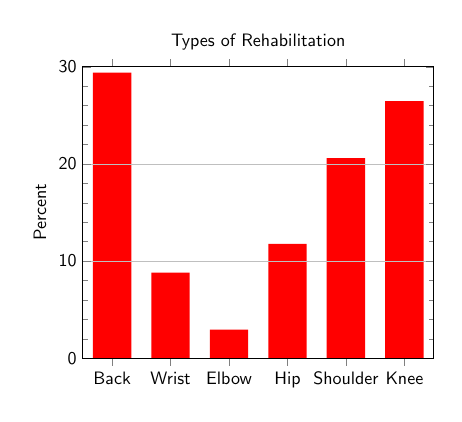
\begin{tikzpicture}[scale=0.65]
    \begin{axis}[
    ybar, axis on top, title={Types of Rehabilitation}, bar width = 0.75cm, ymajorgrids,
    ymin = 0, ymax = 30, ylabel = {Percent}, minor y tick num = 4,
    symbolic x coords = {Back, Wrist, Elbow, Hip, Shoulder, Knee}, xtick=data
    ]
    \addplot [draw=none, fill=red] coordinates{
    (Back, 29.41)
    (Wrist, 8.82)
    (Elbow, 2.94)
    (Hip, 11.76)
    (Shoulder, 20.59)
    (Knee, 26.47)
    };
\end{axis}
\end{tikzpicture}
    \item 5
    \item 5
    \item 30\%
    \item \mbox{} \newline\\
    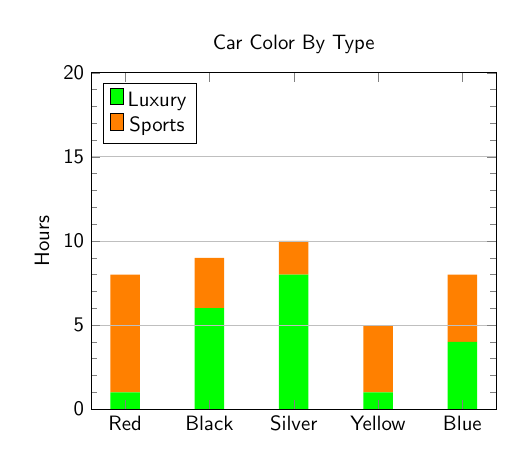
\begin{tikzpicture}[scale=0.75]
    \begin{axis}[
    ybar stacked, axis on top, title={Car Color By Type}, bar width = 0.5cm, ymajorgrids,
    ymin = 0, ymax = 20, ylabel = {Hours}, legend entries = {Luxury, Sports}, legend pos = north west,
    symbolic x coords = {Red, Black, Silver, Yellow, Blue}, xtick=data, minor y tick num = 4
    ]
    \addplot [draw=none, fill=green] coordinates{
    	(Red, 1)
    	(Black, 6)
    	(Silver, 8)
    	(Yellow, 1)
    	(Blue, 4)
    };
    \addplot [draw=none, fill=orange] coordinates{
    	(Red, 7)
    	(Black, 3)
    	(Silver, 2)
    	(Yellow, 4)
    	(Blue, 4)
    };
    \end{axis}
    \end{tikzpicture}
\end{enumerate}

\end{document}
